\documentclass{beamer}
% Графика ----------------------------
\usepackage{graphicx} 
% Математика -------------------------
\usepackage{cmap} 
\usepackage{amsmath}
% Русский язык -----------------------
\usepackage[utf8]{inputenc} 
\usepackage[T2A]{fontenc}
\usepackage[russian]{babel}

% Для включение определенной лекции
\includeonlylecture{lec1}


% Размер сторон:
% ширина – 128 мм, высота – 96 мм (соотношение сторон 4:3).
\title{Искусственные нейронные сети}
\author[Даниил Копылов]{Копылов Д.Е., Михайлов А.А.}
% \date{}
\institute[ИДСТУ СО РАН, ИСП РАН, ИМИТ ИГУ]{
\inst{1}Институт динамики систем и теории управления им. В.М. Матросова Сибирского отделения Российской академии наук \and
\inst{2}Институт системного программирования им. В.П. Иванникова \\Российской академии наук \and
\inst{3}Институт математики и информационных технологий \\Иркутский государственный университет
}

%\insertauthor, \insertdate, \insertinstitute, \inserttitle, \insertsubtitle и \inserttitlegraphic

\begin{document}
\begin{frame}
    \maketitle
\end{frame}

\lecture[История развития]{Предпосылки и история искусственных нейронных сетей}{lec1}
\begin{frame}{Лекция 1}

\insertlecture
% \insertshortlecture %короткое название лекции
\end{frame}
\section{Предпосылки}

\begin{frame}{Древние мифы}
    \begin{figure}[h]
    \begin{center}
    \begin{minipage}[h]{0.6\linewidth}
    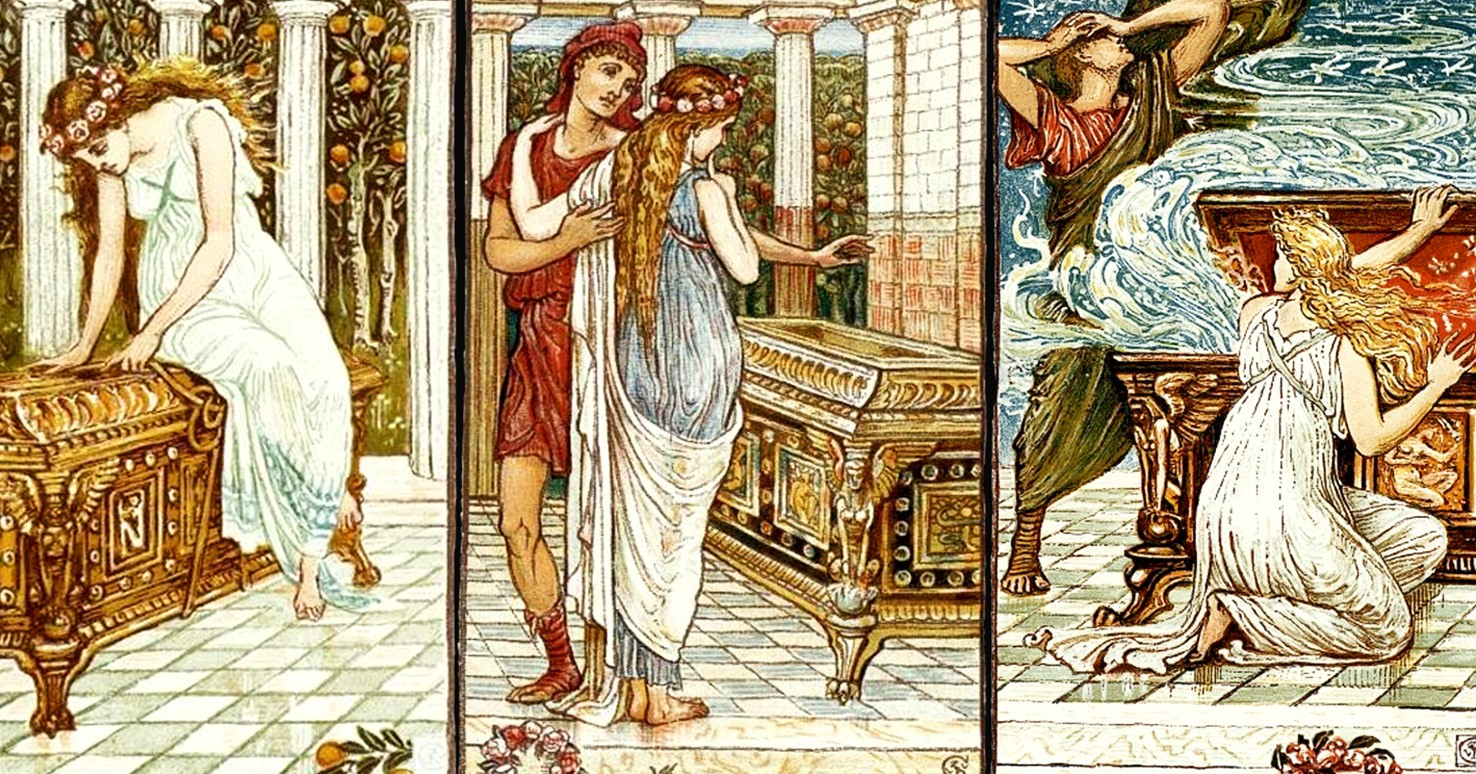
\includegraphics[width=1\linewidth]{img/pandora.jpg}
    \caption{Пандора \\(Древняя Греция) \\кукла, оживленная богами} %% подпись к рисунку
    \label{ris:experimoriginal} %% метка рисунка для ссылки на него
    \end{minipage}
    \hfill
    \begin{minipage}[h]{0.35\linewidth}
    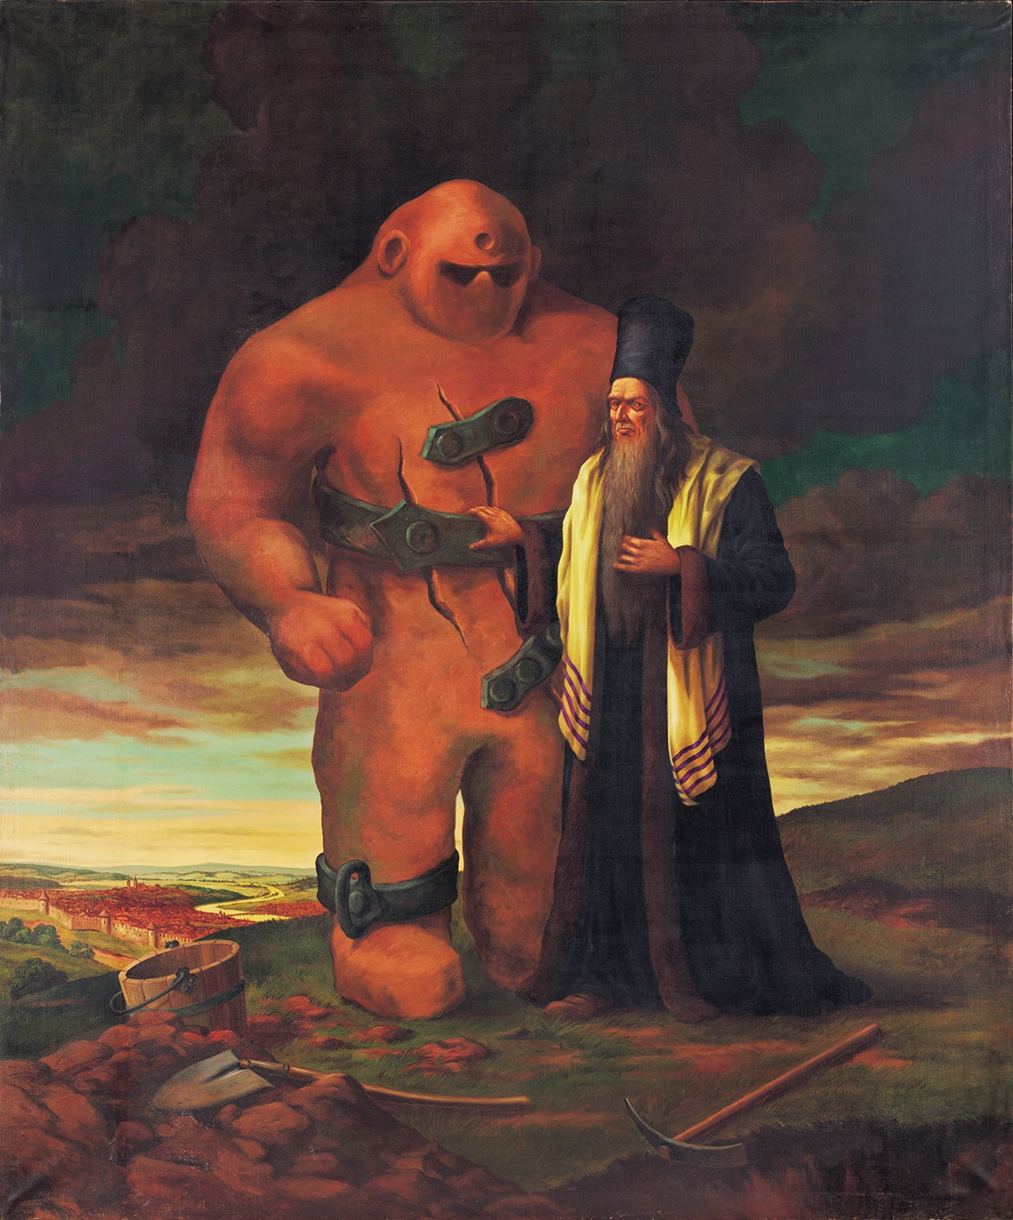
\includegraphics[width=1\linewidth]{img/golem.jpg}
    \caption{Голем \\(еврейская культура) \\мистическое существо из неживой материи}
    \label{ris:experimcoded}
    \end{minipage}
    \end{center}
    \end{figure}
\end{frame}

\begin{frame}{Философские идеи}

\begin{itemize}
    \item \textbf{Рене Декарт (1596-1650)}\\
        Выделение понятия мышление\\
        «Я мыслю, следовательно, я существую»
            
    \item \textbf{Джон Локк (1632-1704)}\\
        Идея, что разум - это чистый лист \\
        «Девять десятых людей делаются такими, какие они есть, только благодаря воспитанию»
        
    \item \textbf{Готфрид Лейбниц (1646-1716)}\\
        Идея описания мышления математикой (мат. логика)\\
        В работе "Искусство комбинаторики"
\end{itemize}
\end{frame}

\section{Биология нейронных сетей}
\begin{frame}{Биология нейрона}

\begin{center}
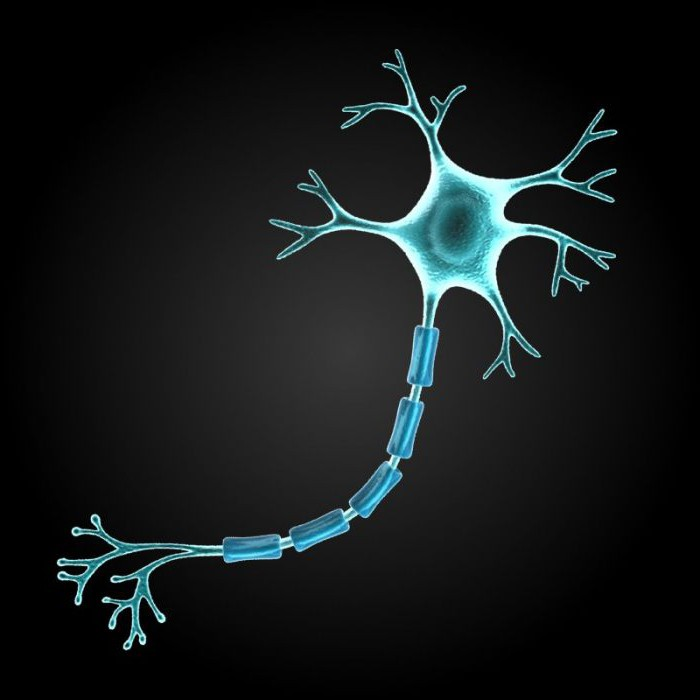
\includegraphics[width=0.5\textwidth]{img/neyron.jpg}
\end{center}
\begin{itemize}
            \item \textbf{Тело нейрона} - содержит ядро и другие органеллы
            \item \textbf{Дендрит}  - принимает сигналы от других нейронов
            \item \textbf{Аксон}  - передает сигналы другим нейронам
        \end{itemize}
\end{frame}
\begin{frame}{Биология искусственного нейрона}
\begin{center}
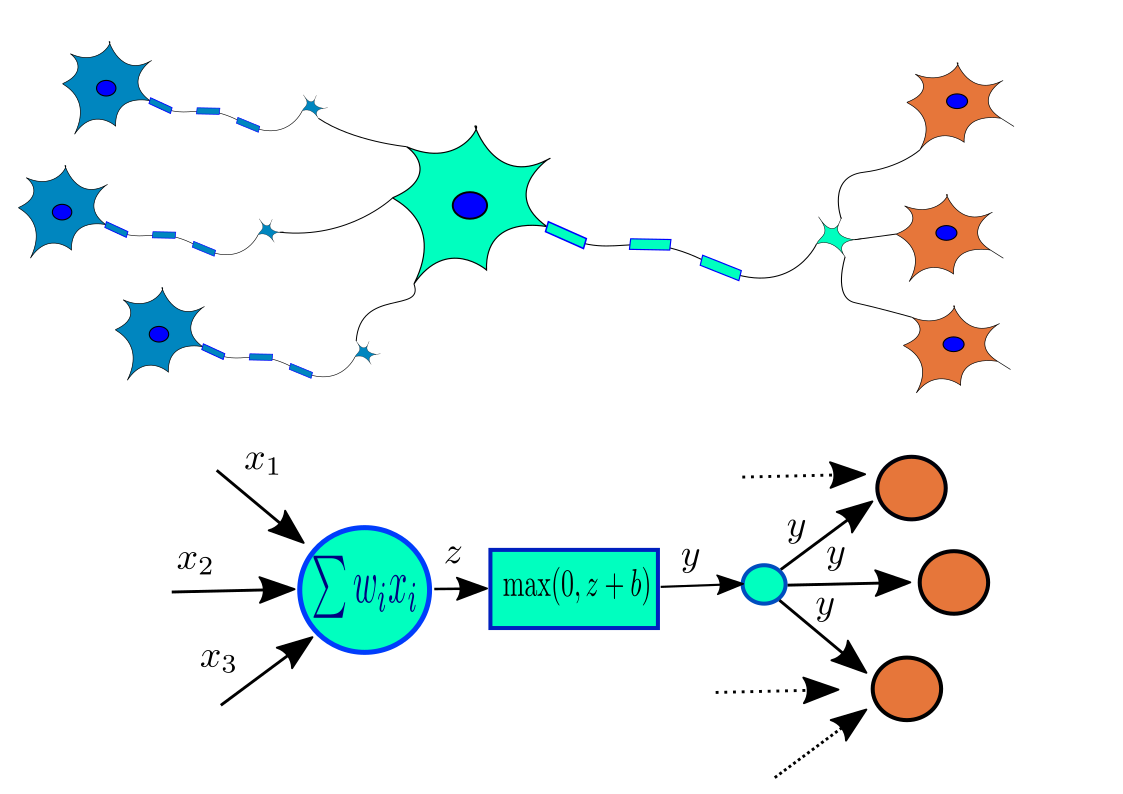
\includegraphics[width=1.0\textwidth]{img/schema.png}
\end{center}
\end{frame}
\section{История искусственных нейронных сетей}
\begin{frame}{Основные этапы развития ИНС}




\begin{itemize}
\item 1940-е - 1960-е годы: зарождение и становление ИНС.
\item 1960-е - 1980-е годы: разочарование в ИНС.
\end{itemize}



\begin{itemize}
\item 1980-е - 2000-е годы: возрождение ИНС.
\item 2000-е годы - настоящее время: расцвет ИНС.
\end{itemize}


\end{frame}
\subsection{Основные этапы}

\begin{frame}{Основные работы}
\begin{center}
\begin{tabular}{|p{0.4in}|p{1.5in}|p{1.3in}|}\hline
\textbf{Год}& \textbf{Архитектура} & \textbf{Автор} \\
\hline
1958 & \textbf{Perceptrons} & Frank Rosenblatt \\\hline
1958 & \textsf{Feed forward neural networks, FF or FFNN} & Frank Rosenblatt \\\hline
1982 & \textsf{Hopfield network} & John J. Hopfield \\\hline
1982 & \textsf{Kohonen networks, KN} & Teuvo Kohonen \\\hline
1986 & \textsf{Boltzmann machines, BM} & Geoffrey E. Hinton, Terrence J. Sejnowski \\\hline
\end{tabular}
\end{center}
\end{frame}

\begin{frame}{Основные работы}
\begin{center}
\begin{tabular}{|p{0.4in}|p{1.5in}|p{1.3in}|}\hline
\textbf{Год}& \textbf{Архитектура} & \textbf{Автор} \\
\hline
1986 & R\textsf{estricted Boltzmann machine, RBM} & Paul Smolensky \\\hline
1988 & \textsf{radial basis function, RBF} & David S. Broomhead, David Lowe \\\hline
1988 & \textbf{Autoencoders, AE} & Hervé Bourlard, Yves Kamp \\\hline
1998 & \textbf{convolutional neural networks, CNN} & Yann LeCun, et al. \\\hline
1990 & \textbf{Recurrent neural networks, RNN} & Jeffrey L. Elman \\\hline
\end{tabular}
\end{center}
\end{frame}

\begin{frame}{Основные работы}
\begin{center}
\begin{tabular}{|p{0.4in}|p{1.5in}|p{1.3in}|}\hline
\textbf{Год}& \textbf{Архитектура} & \textbf{Автор} \\
\hline
1995 & \textsf{Support vector machine, SVM} & Corinna Cortes, Vladimir Vapnik \\\hline
1997 & \textbf{Long short term memory, LSTM} & Sepp Hochreiter, Jürgen Schmidhuber \\\hline
1997 & \textsf{Bidirectional recurrent neural networks (BiRNN, BiLSTM, BiGRU)} & Mike Schuster, Kuldip K. Paliwal \\\hline
2002 & \textbf{Liquid state machines, LSM} & Wolfgang Maass, Thomas Natschläger, Henry Markram \\\hline
2004 & \textbf{Echo state networks, ESN} & Herbert Jaeger, Harald Haas \\\hline
\end{tabular}
\end{center}
\end{frame}

\begin{frame}{Основные работы}
\begin{center}
\begin{tabular}{|p{0.4in}|p{1.5in}|p{1.3in}|}\hline
\textbf{Год}& \textbf{Архитектура} & \textbf{Автор} \\
\hline
2007 & \textsf{Sparse autoencoder, AE} & Marc’Aurelio Ranzato, Christopher Poultney, Sumit Chopra, Yann LeCun \\\hline
2007 & \textsf{Deep belief networks, DBN} & Yoshua Bengio, et al. \\\hline
2008 & \textsf{Denoising autoencoders, DAE} & Pascal Vincent, et al. \\\hline
2010 & \textsf{Deconvolutional networks, DN} & Matthew D. Zeiler, et al. \\\hline
2013 & \textsf{Variational autoencoders (VAE)} & Diederik P. Kingma, Max Welling \\\hline
2013 & \textsf{Extreme learning machines (ELM)} & Erik Cambria, et al. \\\hline
\end{tabular}
\end{center}
\end{frame}

\begin{frame}{Основные работы}
\begin{center}
\begin{tabular}{|p{0.4in}|p{1.5in}|p{1.3in}|}\hline
\textbf{Год}& \textbf{Архитектура} & \textbf{Автор} \\
\hline
2014 & \textsf{Markov chains, MC или discrete time Markov Chain, DTMC} & Brian Hayes \\\hline
2014 & \textbf{Generative adversarial networks, GAN} & Ian Goodfellow, et al. \\\hline
2014 & \textsf{Gated recurrent units, GRU} & Junyoung Chung, et al. \\\hline
2014 & \textbf{Neural Turing machines, NMT} & Alex Graves, Greg Wayne, Ivo Danihelka \\\hline
\end{tabular}
\end{center}
\end{frame}

\begin{frame}{Основные работы}
\begin{center}
\begin{tabular}{|p{0.4in}|p{1.5in}|p{1.3in}|}\hline
\textbf{Год}& \textbf{Архитектура} & \textbf{Автор} \\
\hline
2015 & \textsf{Deep convolutional inverse graphics networks, DCIGN} & Tejas D. Kulkarni, et al. \\\hline
2015 & \textsf{Deep residual networks, DRN} & Kaiming He, et al. \\\hline
2015 & \textbf{Attention networks (AN)} & Max Jaderberg, et al. \\\hline
2016 & \textsf{Differentiable Neural Computers (DNC)} & Alex Graves, et al. \\\hline
2017 & \textsf{Capsule Networks (CapsNet)} & Sara Sabour, Nicholas Frosst, G. E. Hinton \\\hline
\end{tabular}
\end{center}
\end{frame}


\begin{frame}{Значимые события последних лет}
\begin{center}
\begin{tabular}{|p{0.4in}|p{3.5in}|}\hline
\textbf{Год}& \textbf{Событие} \\
\hline
2013 & \textsf{word2vec привносит контекст в слова и фразы, делая еще один шаг в сторону понимания их смысла} \\\hline
2013 & \textsf{уровень ошибок при распознавании речи снизился на 25 \%} \\\hline
2014 & \textsf{Skype переводит речь в режиме реального времени} \\\hline
2014 & \textsf{Чат-бот Юджина Густмана (Eugene Goostman) преодолевает тест Тьюринга} \\\hline
2015 & \textsf{Обученная 1000-слойная сеть Microsoft ResNet превзошла человека в распознавании
изображений} \\\hline
2016 & \textsf{AlphaGo побеждает профессиональных игроков в го} \\\hline
\end{tabular}
\end{center}
\end{frame}

\begin{frame}{Значимые события последних лет}
\begin{center}
\begin{tabular}{|p{0.4in}|p{3.5in}|}\hline
\textbf{Год}& \textbf{Событие} \\
\hline
2016 & \textsf{Microsoft достигает человеческого уровня в распознавании разговорной речи} \\\hline
2017 & \textsf{AlphaGo Zero самостоятельно обучается игре в го за 3 дня} \\\hline
2018 & \textsf{Deep Fakes заменяет одно лицо другим в видео} \\\hline
2018 & \textsf{Нейронная сеть BERT компании Google помогает людям переводить с одного языка
на другой} \\\hline
2019 & \textsf{OpenAI Five сокрушает чемпионов мира в игре Dota2} \\\hline
2019 & \textsf{OpenAI GPT-2 генерирует реалистичные отрывки текста} \\\hline
\end{tabular}
\end{center}
\end{frame}


\begin{frame}{Зоопарк нейронных сетей}
\begin{center}
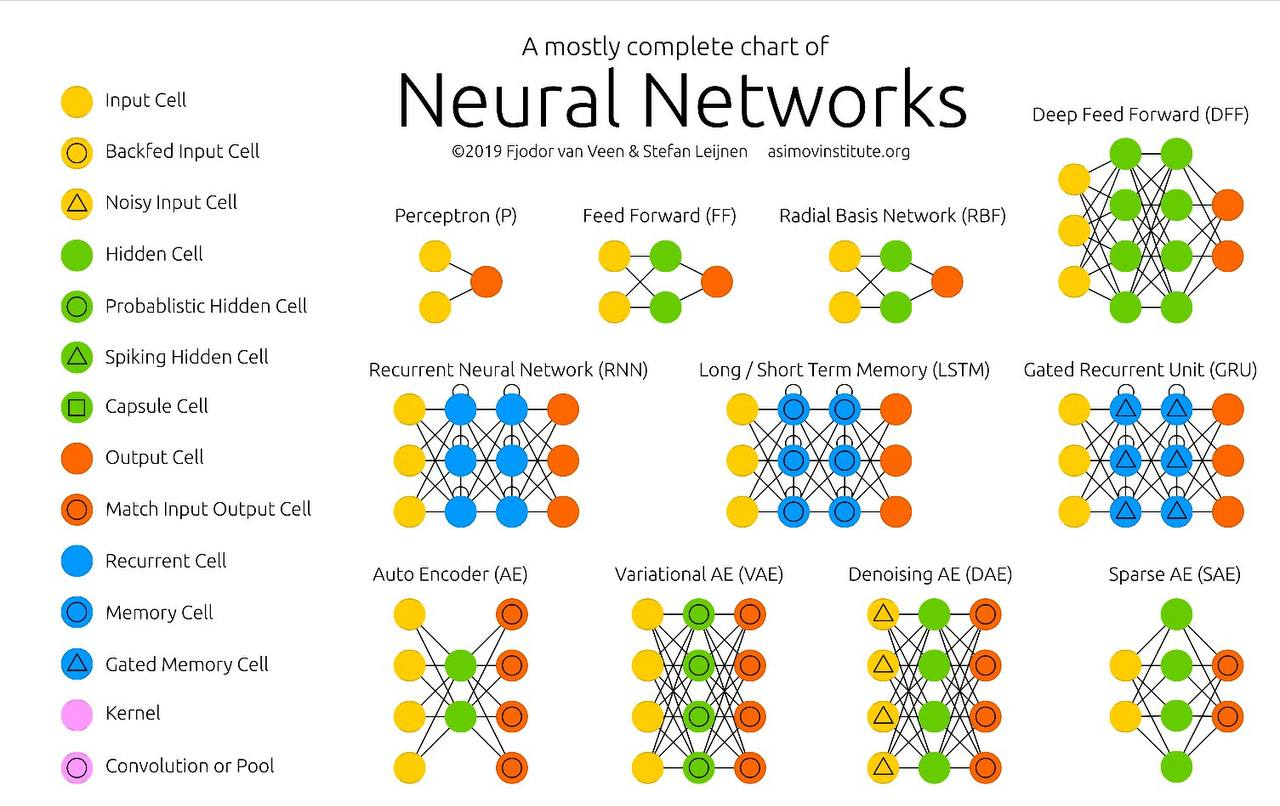
\includegraphics[width=1.0\textwidth]{img/a1.jpg}
\end{center}
\end{frame}

\begin{frame}{Зоопарк нейронных сетей}
\begin{center}
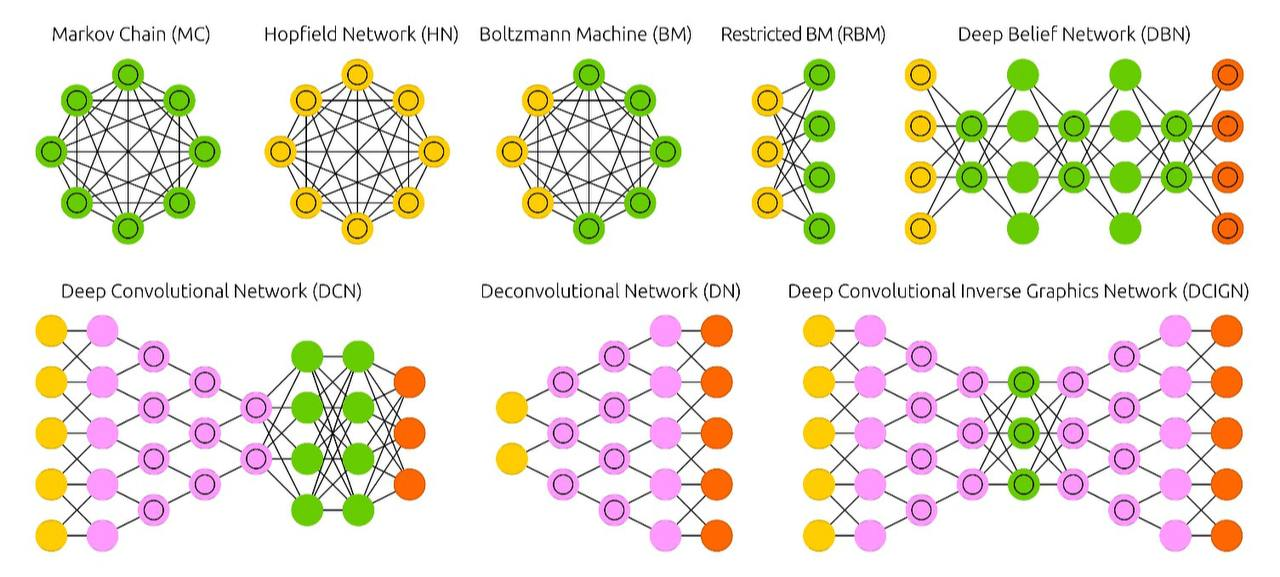
\includegraphics[width=1.0\textwidth]{img/a2.jpg}
\end{center}
\end{frame}

\begin{frame}{Зоопарк нейронных сетей}
\begin{center}
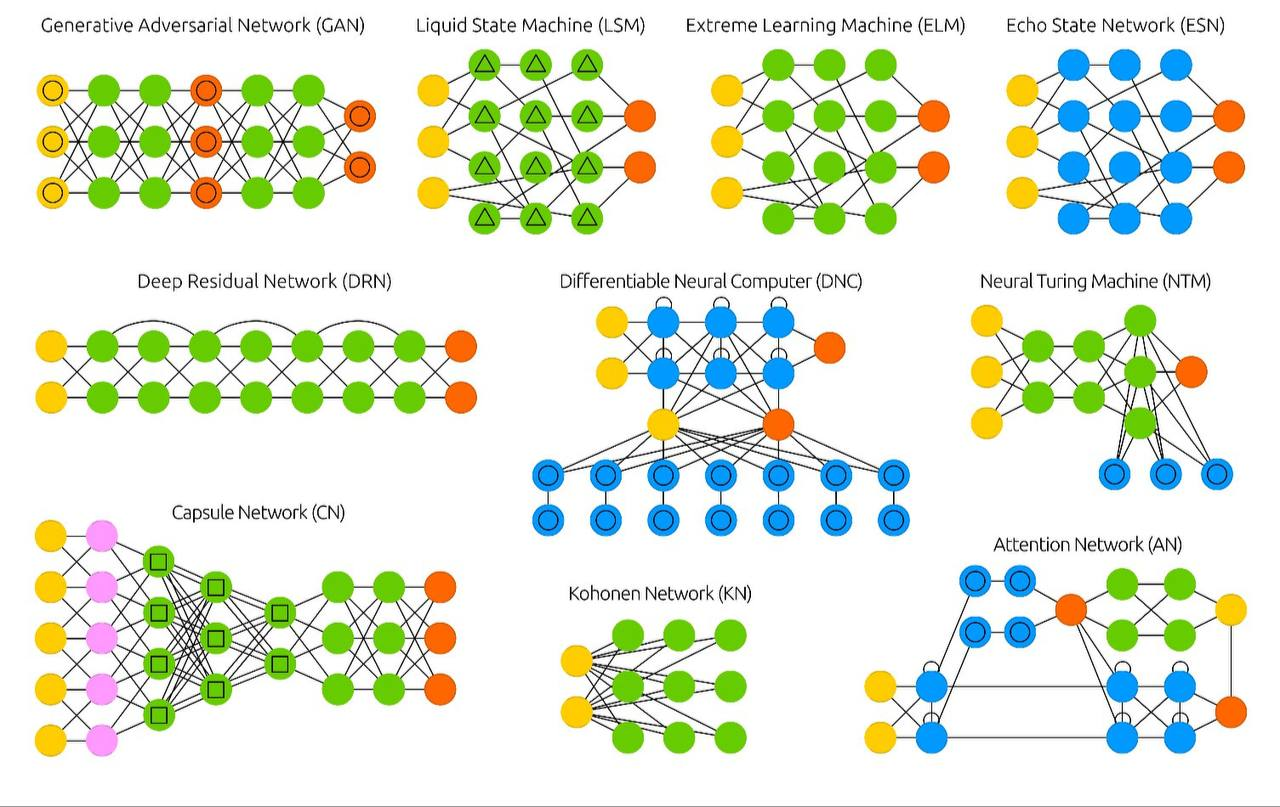
\includegraphics[width=1.0\textwidth]{img/a3.jpg}
\end{center}
\end{frame}

\section{Классификация}


\begin{frame}{Классификация по задачам}


\begin{itemize}
\item Классификация
\item Преобразование типов
\item Аугментация данных
\item Выделение признаков
\item Генерация
\item Поиск
\end{itemize}
\end{frame}

\begin{frame}{Классификация по технологиям}


\begin{itemize}
\item Сверточные нейронные сети (CNN)
\item Рекуррентные нейронные сети (RNN)
\item Генеративные нейронные сети (GAN)
\item Автоэнкодеры
\end{itemize}
\end{frame}

\begin{frame}{Классификация по сферам применения}


\begin{itemize}
\item Бизнес
\item Наука
\item Искусство
\item Развлечение
\end{itemize}
\end{frame}

\begin{frame}{Классификация по типу данных}

\begin{itemize}
\item Цифры
\item Изображения
\item Речь
\item Видео
\item Текст
\end{itemize}
\end{frame}
\subsection{Ключевые технологии}

\begin{frame}{Perceptrons}


\begin{itemize}
\item Простейшая нейронная сеть, состоящая из одного слоя нейронов.
\item Каждый нейрон имеет один вход и один выход.
\item Вход представляет собой значение одного элемента входного набора данных, а выход представляет собой значение одного элемента выходного набора данных.
\end{itemize}
\end{frame}

\begin{frame}{Direct Feed-Forward}


\begin{itemize}
\item Нейронная сеть, в которой все нейроны в одном слое напрямую связаны с нейронами в следующем слое.
\item DFF-сети являются одними из самых простых и эффективных нейронных сетей.
\item Используются для решения широкого круга задач, включая классификацию, регрессию и кластеризацию.
\end{itemize}
\end{frame}

\begin{frame}{Autoencoder}


\begin{itemize}
\item Нейронная сеть, которая кодирует входное значение в скрытое представление, а затем декодирует скрытое представление обратно в выходное значение.
\item Автокодировщики используются для обучения представления данных.
\item Могут использоваться для снижения размерности данных, улучшения качества изображений и обнаружения аномалий.
\end{itemize}
\end{frame}

\begin{frame}{Boltzmann Machine}


\begin{itemize}
\item Вероятностная модель, основанная на нейронных сетях.
\item BM-модели используются для моделирования сложных систем, таких как природные языки и социальные сети.
\end{itemize}
\end{frame}

\begin{frame}{Deep Convolutional Neural Network}


\begin{itemize}
\item Нейронная сеть, которая использует сверточные операции.
\item Сверточные операции позволяют DCN-сетям эффективно обрабатывать данные, имеющие пространственную структуру, такие как изображения и видео.
\item DCN-сети используются для решения широкого круга задач, включая распознавание изображений, машинный перевод и компьютерное зрение.
\end{itemize}
\end{frame}

\begin{frame}{Attention Network}


\begin{itemize}
\item Нейронная сеть, которая использует внимание для обработки информации.
\item Внимание позволяет AN-сетям фокусироваться на важных частях входного набора данных.
\item AN-сети используются для решения широкого круга задач, включая машинный перевод, компьютерное зрение и обработка естественного языка.
\end{itemize}
\end{frame}

\lecture[Классификаци]{Классификаци}{lec2}{}



\begin{frame}{Лекция 2}

\end{frame}

\end{document}
